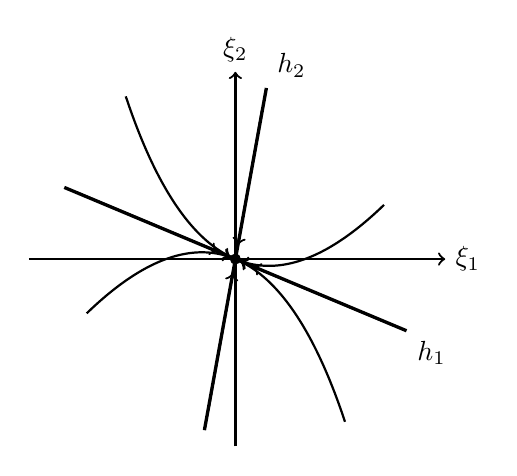
\begin{tikzpicture}[x=0.82cm,y=0.82cm,thick]
  % Stable node in a skew eigenbasis; h1 is the slow direction.
  \draw[->] (-3.2,0)--(3.25,0) node[right] {$\xi_1$};
  \draw[->] (0,-2.9)--(0,2.9) node[above] {$\xi_2$};
  \draw[very thick] (-2.65,1.11)--(2.65,-1.11) node[below right] {$\vect{h}_1$};
  \draw[very thick] (-0.48,-2.65)--(0.48,2.65) node[above right] {$\vect{h}_2$};
  \draw[->] (-2.45,1.03)--(-0.28,0.12); \draw[->] (2.45,-1.03)--(0.28,-0.12);
  \draw[->] (-0.42,-2.35)--(-0.04,-0.22); \draw[->] (0.42,2.35)--(0.04,0.22);
  % Plot v = C u^2 in eigen-coordinates, then shear it into the physical plane.
  \foreach \su in {-1,1} {\foreach \sv in {-1,1} {
    \draw[->] plot[domain=2.0:0.08,samples=65,variable=\s]
      ({\su*\s+0.18*\sv*0.42*\s*\s},{-0.42*\su*\s+\sv*0.42*\s*\s});
  }}
  \fill (0,0) circle (2pt);
\end{tikzpicture}
